\Chapter{Szimulációk}

\Section{Szimuláció program}
A szimulációk elvégzéséhez egy külön programot hoztam létre, amelyben a különböző AI-okat játszattam egymás ellen. Ezeknek a szimulációknak az eredményét kezdetben a konzolra írtam ki, hogy fel tudjam mérni a különböző AI-ok képességeit.

\SubSection{Első AI a második AI ellen}
A szimulációk elvégeztével egyértelműen látszott, hogy a második sokkal eredményesebb mint az első, hiszen általánosan körülbelül a 85\%-át tudta megnyerni a lejátszott játékoknak.\par
Különböző vizsgálatokat futtattam a két AI játszmáinak kapcsán. Először azt vizsgáltam, hogy milyen a lejátszott meccsek végén a játékosok összpontszámainak gyakoriság hisztogramja tízezer játék esetén.

\begin{figure}[h]
\centering
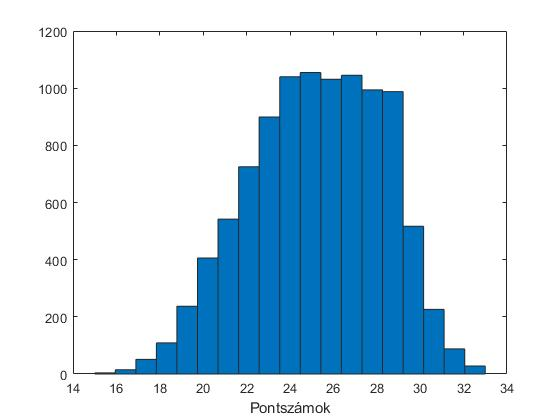
\includegraphics[scale=0.6]{images/final_scores_AI1vsAI2.jpg}
\caption{Az első és második AI összpontszámainak eloszlása.}
\label{fig:scores1v2}
\end{figure}

\newpage
Egy hasonló vizsgálat során, ugyanezen játékszám mellett a lejátszott meccsek köreinek számát tekintve vizsgáltam meg a gyakoriság hisztogramját.

\begin{figure}[h]
\centering
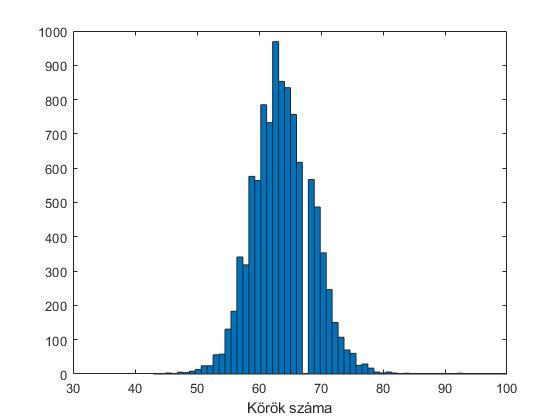
\includegraphics[scale=0.5]{images/round_number_hist_AI1vsAI2.jpg}
\caption{Az első és második AI köreinek eloszlása.}
\label{fig:rounds1v2}
\end{figure}

Végezetül pedig egy játékban a pontszámaiknak növekedését tekintettem.
\begin{figure}[h]
\centering
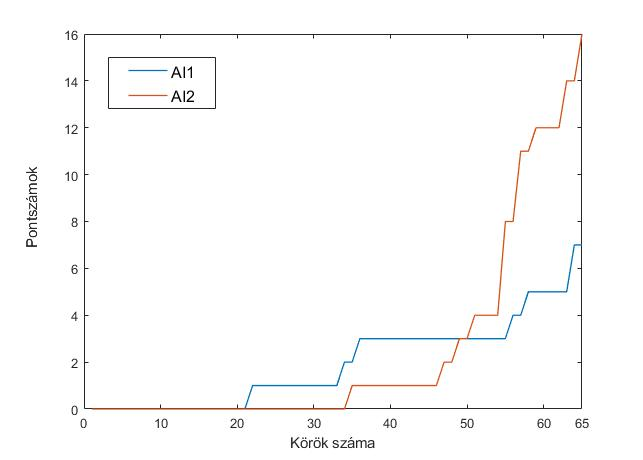
\includegraphics[scale=0.5]{images/player_points_AI1vsAI2.jpg}
\caption{Az első és második AI pontszámainak növekedése.}
\label{fig:player_scores1v2}
\end{figure}


\SubSection{Második AI a harmadik AI ellen}

Ahogy elvégeztem a szimulációkat, kiderült, hogy a második logika kicsivel nagyobb arányban tudott nyerni, mint a harmadik. Az, hogy nem hatékony abból fakad, hogy a játék előrehaladtával a késői fázisban is csak azt nézi, hogy melyik a számára legkönnyebben elérhető lap, így az alacsony szintűekre kezd el gyűjteni, nem pedig az értékesebb lapokra, így a pontszerzés a háttérbe szorul és a másik logika felé tud kerekedni.

\SubSection{Második AI a negyedik AI ellen}

A negyedik AI elkészítése után lefuttatva a szimulációkat kiderült, hogy a negyedik algoritmus körülbelül annyival erősebb, mint amennyivel a második volt az elsőtől. Általánosan 86\%-kát nyeri meg a lejátszott játékaiknak. Ez bizonyult tehát a legeredményesebb logikának a szimulációim során.\par

Az elsőhöz hasonlóan megnéztem, hogy miként alakul a játékok végén a játékosok összpontszámainak gyakoriság hisztogramja szintén tízezer játszma esetén.

\begin{figure}[h]
\centering
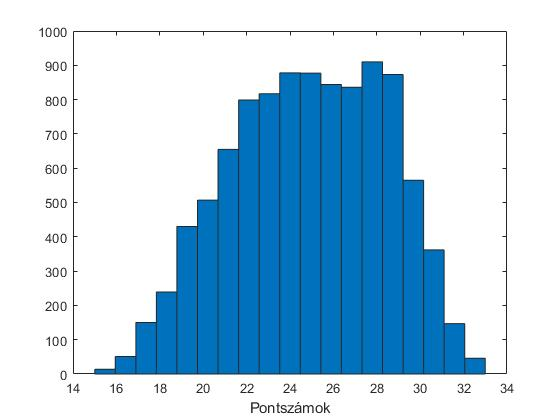
\includegraphics[scale=0.55]{images/final_scores_AI2vsAI4.jpg}
\caption{A második és negyedik AI összpontszámainak eloszlása.}
\label{fig:scores2v4}
\end{figure}

A következő vizsgálat során tízezer játékszám mellett a lejátszott meccsek köreinek számát tekintve vizsgáltam meg a gyakoriság hisztogramját, ahogy korábban is tettem.

\begin{figure}[h]
\centering
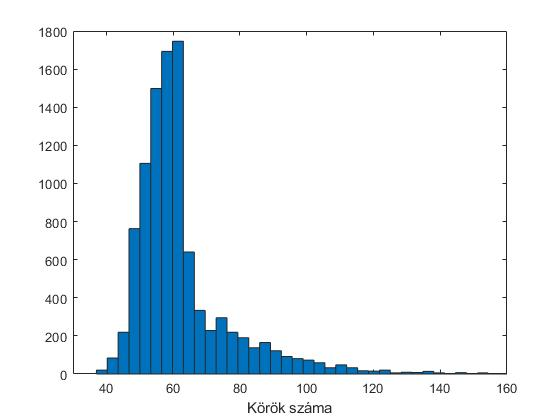
\includegraphics[scale=0.55]{images/round_number_hist_AI2vsAI4.jpg}
\caption{A második és negyedik AI köreinek eloszlása.}
\label{fig:rounds2v4}
\end{figure}

Ezután pedig az egy játékban való pontjaiknak a növekedését is szintén megvizsgáltam.

\begin{figure}[h]
\centering
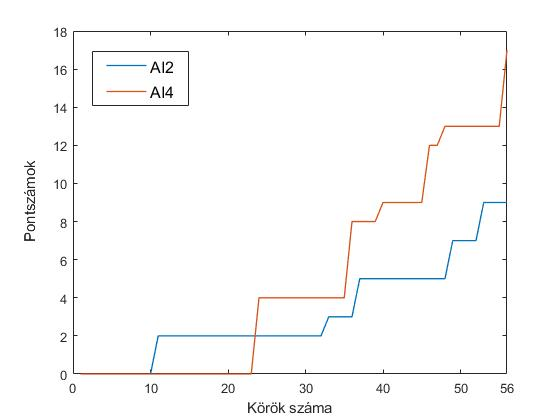
\includegraphics[scale=0.6]{images/player_points_AI2vsAI4.jpg}
\caption{Az első és második AI pontszámainak növekedése.}
\label{fig:player_scores2v4}
\end{figure}


